\begin{figure}[t]
    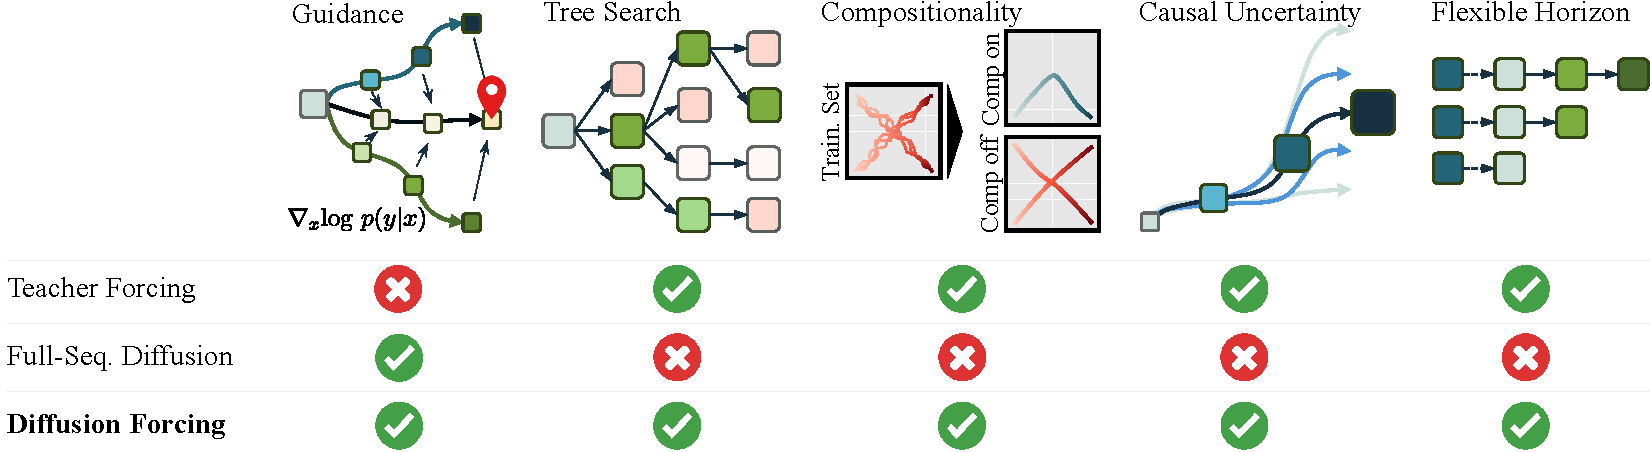
\includegraphics[width=\linewidth]{figures/pdf/Capabilities.pdf}
    \caption{\textbf{\algo{} capabilities.} Today, different applications such as language modeling~\cite{gpt3}, planning~\cite{janner2022planning}, or video generation~\cite{ho2022video,yang2023diffusion} rely on \emph{either} auto-regressive next-token prediction \emph{or} full-sequence diffusion, according to their respective unique capabilities. The proposed \algons{} is a novel sequence generative model that enjoys key strengths of both model types.} 
    \label{fig:ability}
    \vspace{-5pt}
\end{figure}
